\chapter{Projektplan}
Nach der Einfindung der Projektgruppe in das allgemeine Thema wird relativ früh ein grober Projektplan entworfen, um den Ablauf des Projektes zu erfassen und mögliche Abhängigkeiten zu identifizieren. Bei diesem ersten Entwurf werde daher vorerst nur sehr grobe Aufgabenpakete entworfen, welche über den Verlauf der Projektgruppe weiter ausgearbeitet werden oder gegebenenfalls angepasst werden müssen.

\section{Erklärung des Projektplans}
Der Projektplan in \Fig{Projektplan} stellt die groben Arbeitspakete mit ihren Start- und geplanten Enddatum dar. 

\subsection{Einteilung der Arbeitspakete}
Die Aufgabenpakete können nach dem Vorgehensmodell aus dem vorherigen Kapitel in zwei Kategorien eingeteilt werden:
\begin{enumerate}
	\item Definitionsphase 
	\item Implementierungsphase
\end{enumerate}
Während die ersten Aufgabenpakete Visionsdokument erstellt, Projekthandbuch erstellt, Anforderungsanalyse erstellt, Architektur erstellt und Seminarvorträge gehalten zu der sogenannten Definitionsphase gehören, kann der Prototyp des Schülerinformationstages, die internen Praktika zur Vorbereitung der Implementierung, die Meilensteine 1 bis 5 und die Evaluation und Nachbereitung in die Implementierungsphase kategorisiert werden.

\begin{figure}[!ht]
	\centering
	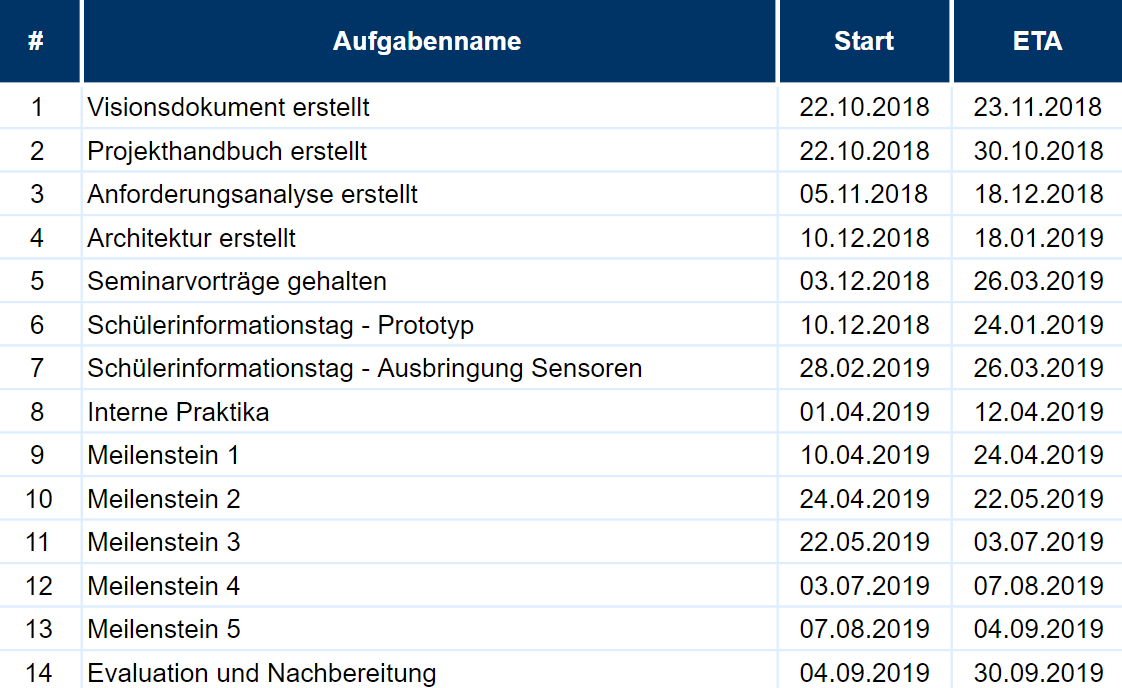
\includegraphics[width=\textwidth]{./ressourcen/projektplan.png}
	\caption{Grober Projektplan}
	\label{fig:Projektplan}
\end{figure}

\subsection{Abweichungen des Projektplans}
Wie bereits in der Einleitung des Projektplans erwähnt, ist es durch einige Ressourcen Verschiebungen, wie z.B. der Schülerinformationstag, zur nicht Einhaltung des Enddatums von einigen vorherigen Arbeitspaketen gekommen. An dieser Verfehlung der festgelegten Zeiten waren aber auch zu optimistische Schätzungen und die falsche Einschätzung wie lange die Abnahme von Dokumenten, wie z.B. das Visionsdokument, durch die Betreuer in Anspruch nimmt. Allgemein kann gesagt werden, dass die Abweichung besonders die Arbeitspakete 1, 3 und 4 betreffen, welche statt wie geplant alle Ende Januar abgeschlossen sein sollten sich alle bis in den späten März gezogen haben.

\section{Fazit}
Besonders am Anfang der Projektgruppe wurde der Aufwand der Anforderungsanalyse und Erstellung der Architektur unterschätzt. Dies wurde durch die zusätzliche Inanspruchnahme von Ressourcen durch den Schülerinformationstag intensiviert. Durch die Fehlplanung am Anfang verschob sich die Implementierungsphase zum Start des Sommersemesters 2019 (10.04.2019). Die Implementierungsphase verlief dabei eher nach dem Projektplan, obwohl auch hier teilweise einige Abweichungen existieren, welche jedoch durch den Mangel an Erfahrung selbstverständlich sind. Insgesamt ist festzuhalten, dass die Struktur des Projektplans eingehalten wurde, aber es zeitliche Abweichungen von den ursprünglich geplanten Daten gab.